\documentclass{beamer}
\usepackage[utf8]{inputenc}
\usepackage[italian]{babel}
%Information to be included in the title page:
\title{Approfondimento sulla programmazione a blocchi con Micro:Bit}

\graphicspath{{./media/}}

\begin{document}

\frame{\titlepage}

\begin{frame}
	\frametitle{Introduzione}
	
	\begin{figure}[h]
		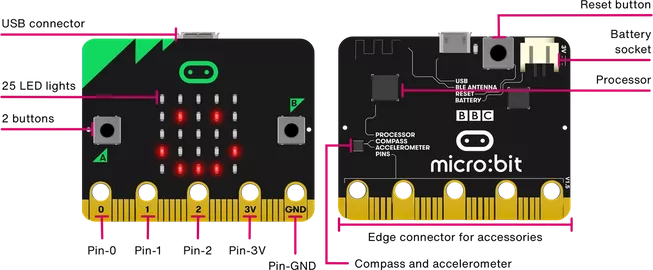
\includegraphics[width=11cm]{mbScheme.png}
	\end{figure}

\end{frame}

\begin{frame}
	\frametitle{Editor}
	
	\begin{center}
		\textbf{https://microbit.org/join}
	\end{center}

	
\end{frame}

\begin{frame}
	\frametitle{Scratch e Make:Code}

	\textit{Quali sono le similitudini e quali le differenze tra Scratch e Make:Code?}

\end{frame}

\begin{frame}
	\frametitle{Attività 1 - Display}
	
	Realizzare un programma che scriva sul display il contenuto di una variabile ti tipo stringa.

	\vspace{2em}
	\begin{enumerate}
		\item Inizializzare la variabile con un valore
		\item Visualizzare il valore
	\end{enumerate}

	\vspace{2em}
	\textit{C'è differenza tra come viene visualizzata una stringa composta da un solo carattere e una stringa composta da più caratteri?}

\end{frame}

\begin{frame}
	\frametitle{Attività 2 - Contatore}

	Realizzare un programma che incrementa o decrementa una variabile di tipo numerico alla pressione di un pulsante e ne visualizza il valore sul display.

	\vspace{2em}
	\begin{itemize}
		\item Il tasto A deve decrementare la variabile di 1
		\item Il tasto B deve incrementare la variabile di 1
		\item (EXTRA) Il valore della variabile deve sempre rimanere compreso tra 0 e 9
	\end{itemize}
	

\end{frame}

\begin{frame}
	\frametitle{Attività 3 - Cronometro}

	Realizzare un cronometro che misuri il tempo trascorso tra la prima e la seconda pressione del pulsante A.

	\vspace{2em}
	\begin{itemize}
		\item La prima pressione del pulsante A deve avviare il cronometro 
		\item La seconda pressione del pulsante A deve fermare il cronometro e mostrare il tempo trascorso sul display in secondi
		\item Il display deve mostrare sempre lo stato attuale del sistema (simbolo attesa, simbolo misurazione, tempo trascorso)
	\end{itemize}
\end{frame}

\begin{frame}
	\frametitle{Attività 4 - Reaction Game 1}
	Realizzare un programma che misuri il tempo di reazione di un giocatore.
	\vspace{2em}
	\begin{enumerate}
		\item Mostrare un simbolo di attesa
		\item Attende un tempo casuale tra 1 e 10 secondi
		\item Mostrare un simbolo di conferma sul display
		\item Misurare quanto tempo passa tra la comparsa del simbolo e la pressione del pulsante A da parte dell'utente
		\item Mostrare il tempo di reazione sul display in millisecondi
		\item (EXTRA) Impedire che il giocatore possa barare premendo il pulsante A prima che il simbolo di conferma sia apparso
	\end{enumerate}	
\end{frame}

\begin{frame}
	\frametitle{Attività 5 - Reaction Game 2}
	Estendere il programma della slide precedente introducendo un secondo giocatore.\\
	
	\vspace{0.5em}
	\begin{enumerate}
		\item Mostrare un simbolo di attesa
		\item Attende un tempo casuale tra 1 e 10 secondi
		\item Mostrare un simbolo sul display
		\item Attende che almeno uno dei due giocatori prema il proprio pulsante
		\item Misurare quanto tempo passa tra la comparsa del simbolo e la pressione di uno dei due pulsanti
		\item Mostrare il giocatore che ha vinto sul display
		\item (EXTRA) Impedire che i giocatori possa barare premendo il pulsante prima che il simbolo di conferma sia apparso
		\item (EXTRA) Mostrare anche lo scarto tra i tempi dei due giocatori (differenza tra i due).
	\end{enumerate}	
\end{frame}

\begin{frame}
	\frametitle{Attività 6 - Livella - Introduzione}

	\begin{figure}[h]
		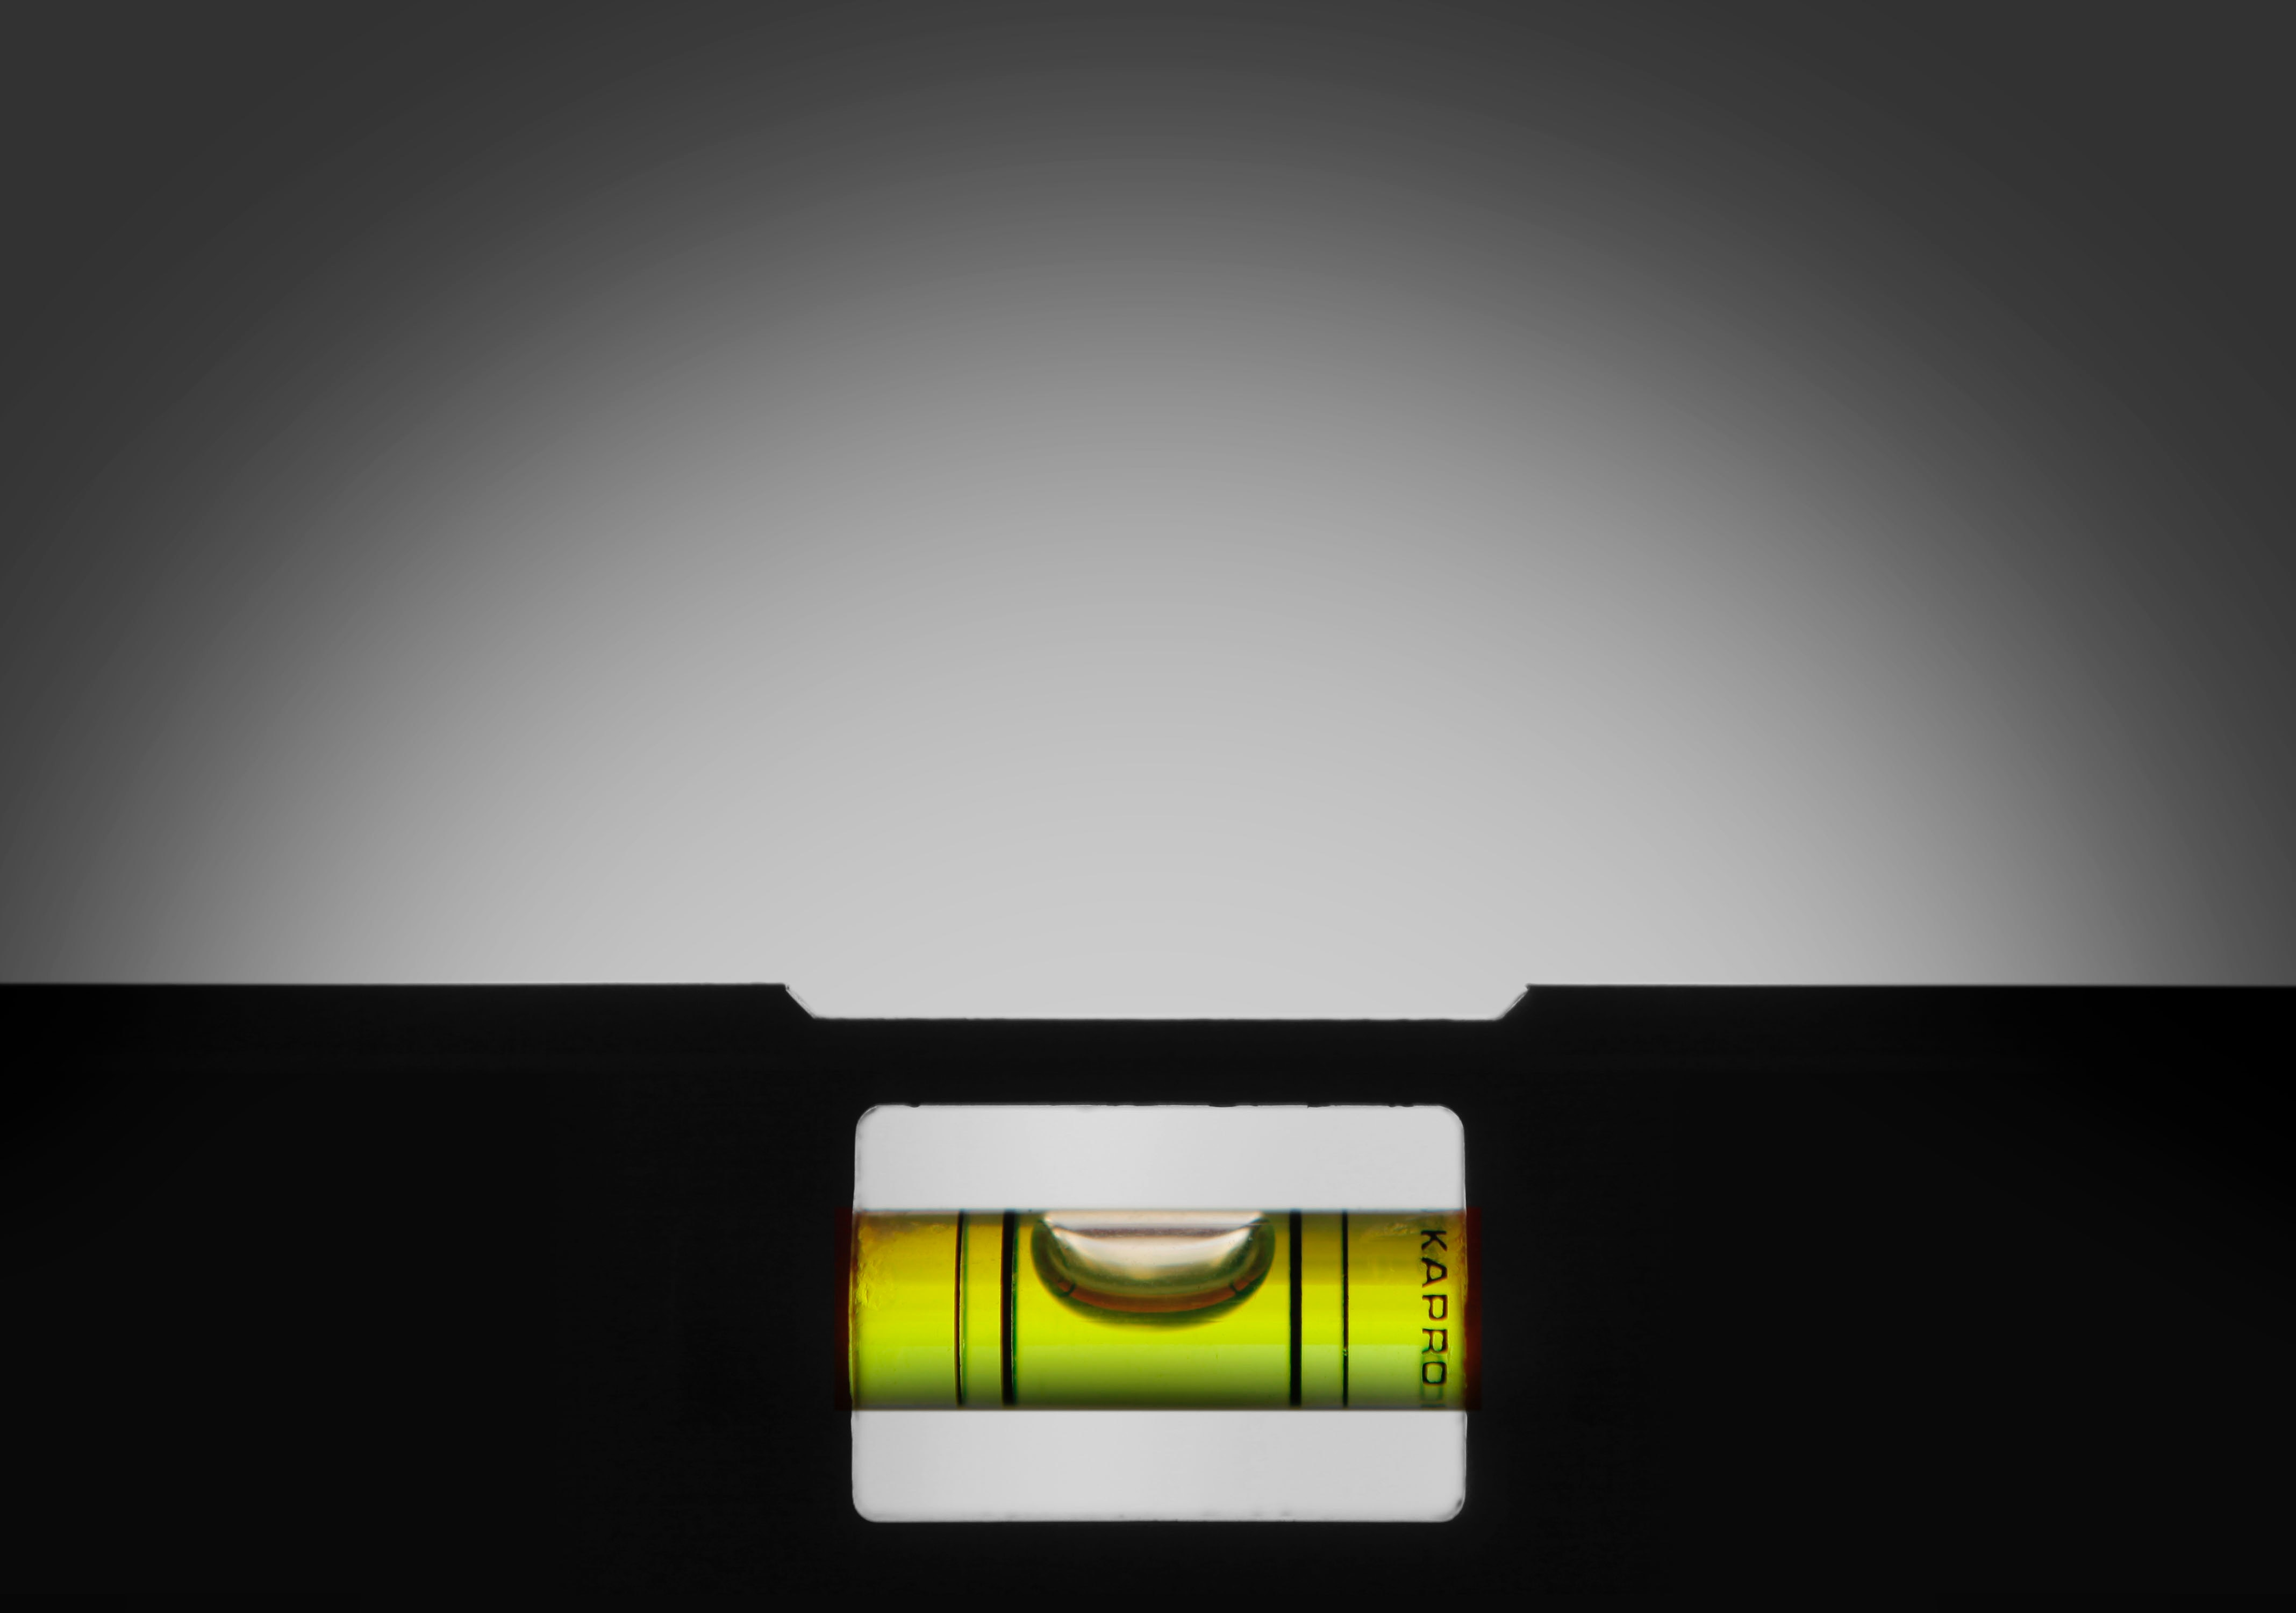
\includegraphics[width=5cm]{level.jpg}
	\end{figure}
	
	La livella è uno strumento che permette di verificare se un piano è orizzontale o meno.\\
	L'oviettivo di questa attività è quello di realizzare una livella digitale con Micro:Bit.

\end{frame}

\begin{frame}
	\frametitle{Attività 6 - Livella - Giroscopio}


	\begin{figure}[h]
		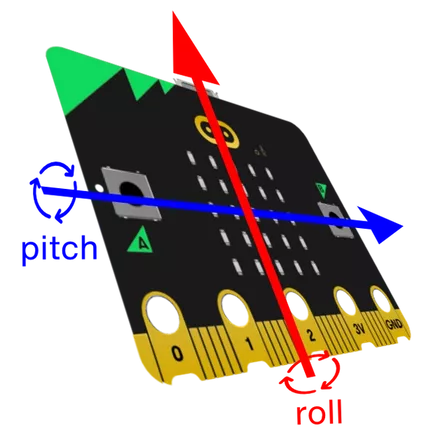
\includegraphics[width=5cm]{mbAxes.png}
	\end{figure}

	Micro:Bit è dotato di un giroscopio che permette di rilevare la rotazione su due assi, noti come \textit{pitch} (\textit{beccheggio}) e \textit{roll} (\textit{rollio}).\\

\end{frame}

\begin{frame}
	\frametitle{Attività 6 - Livella - LED}

	\begin{figure}[h]
		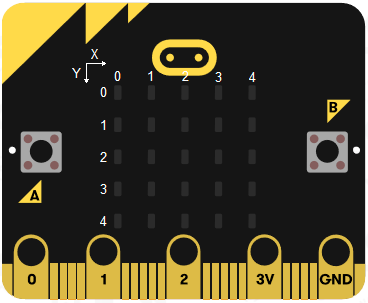
\includegraphics[width=5cm]{mbLedGrid.png}
	\end{figure}

	I led che compongono il display sono disposti in una griglia 5x5 in 0,0 è l'angolo in alto a sinistra.\\
	Fino ad ora abbiamo utilizzato il display come un unico blocco, ma è possibile accendere e spegnere ogni singolo led.

\end{frame}

\begin{frame}
	\frametitle{Attività 6 - Livella}

	\begin{enumerate}
		\item Salvare i valori di rollio e beccheggio su due variabili;
		\item Mappare i valori di rollio e beccheggio sui led della griglia come segue:
		\begin{itemize}
			\item Valori compresi tra -10 e +10 devono essere mappati sul led centrale (Riga o Colonna 2);
			\item Valori compresi tra -20 e -10 devono essere mappati su Riga o Colonna 3;
			\item Valori minori di -20 devono essere mappati su Riga o Colonna 4;
			\item Valori compresi tra +10 e +20 devono essere mappati su Riga o Colonna 1;
			\item Valori maggiori di 20 devono essere mappati su Riga o Colonna 0;
		\end{itemize}
		\item Pulire lo schermo e accendere il LED corrispondente.
		\item (EXTRA) Premendo i tasti A o B consentire di visualizzare le variazioni solo su un asse.
	\end{enumerate}

\end{frame}

\begin{frame}
	\frametitle{Progetti}

	\begin{itemize}
		\item Bussola
		\item Allarme di movimento
		\item Bilancia la biglia
		\item Mini snake
	\end{itemize}
	
\end{frame}

\begin{frame}
	\frametitle{Progetto 1 - Bussola}

	Realizzare una bussola digitale che mostri la direzione in cui si trova il nord magnetico sotto forma di freccia sul display.
	
\end{frame}

\begin{frame}
	\frametitle{Progetto 2 - Allarme di movimento}

	Realizzare un allarme di movimento che scatti quando il Micro:Bit viene spostato.\\
	Lo spostamento deve poter essere rilevato dal giroscopio (sotto forma di rotazione) o dall'accelerometro (sotto forma di accelerazione).\\
	Quando l'allarme scatta, il display deve mostrare un simbolo di allarme lampeggiante.

\end{frame}

\begin{frame}
	\frametitle{Progetto 3 - Bilancia la biglia}

	Realizzare un gioco in cui bisogna portare una biglia in un punto preciso senza farla uscire dallo schermo.\\
	Rappresentare la biglia con un led acceso con intensità massima e l'obiettivo con un led acceso con intensità bassa. Le posizioni di biglia e obiettivo devono essere generate randomicamente.\\
	Utilizzare giroscopio o accellerometro per muovere la biglia. A differenza dell'attivitò sulla livella, i dati del sensore indicheranno come la biglia deve spostarsi invece che la sua posizione\\
	Quando la biglia raggiunge l'obiettivo, il display deve mostrare un simbolo di conferma.\\
	Se la biglia esce dallo schermo, il display deve mostrare un simbolo di errore.	

\end{frame}

\begin{frame}
	\frametitle{Progetto 4 - Mini Snake}

	Realizzare un remake del classico gioco Snake.\\
	La testa del serpente deve essere rappresentata da un led acceso con intensità massima, il corpo da un led acceso con intensità media, l'obiettivo da un led acceso con intensità bassa.\\
	Il cambio di direzione avviene tramite input da giroscopio o accelerometro.\\
	Quando il serpente mangia l'obiettivo, il corpo si allunga di un led.\\
	Se il serpente si morde, il display deve mostrare un simbolo di errore.\\
	Il gioco prosegue finchè il serpente non si morde.

\end{frame}

\begin{frame}
	\frametitle{References}
	\begin{itemize}
		\item \href{https://microbit.org/get-started/user-guide/overview/}{Schema Micro:Bit \textit{https://microbit.org/get-started/user-guide/overview}}
		\item \href{https://unsplash.com/photos/zfVIh4cX_4c}{Immagine Livella \textit{https://unsplash.com/photos/zfVIh4cX\_4c}} 
		\item \href{https://microbit.org/projects/make-it-code-it/spirit-level/}{Assi rotazione Micro:Bit \textit{https://microbit.org/projects/make-it-code-it/spirit-level/}}
		\item \href{https://support.microbit.org/support/solutions/articles/19000127759-micro-bit-led-x-y-orientation}{Schema LED Micro:Bit \textit{https://support.microbit.org/support/solutions/articles/19000127759-micro-bit-led-x-y-orientation}}
	\end{itemize}
\end{frame}
\end{document}